% THIS IS A CHANGE
%%%%%%%%%%%%%%%%%%%%%%%%%%%%%% Preamble
\documentclass{article}
\usepackage{amsmath,amssymb,amsthm,fullpage,float,graphicx,braket,rotating,verbatim}
\newtheorem*{prop}{Proposition}
\newcommand{\e}{\epsilon}
\newcommand{\del}{\partial}
\newcommand{\R}{\mathbb{R}}
\newcommand{\beq}{\begin{equation}}
\newcommand{\eeq}{\end{equation}}
% \newcommand\numberthis{\addtocounter{equation}{1}\tag{\theequation}}
\def\bal#1\eal{\begin{align}#1\end{align}}

\usepackage[usenames,dvipsnames,svgnames,table]{xcolor}
\newcommand{\cdw}[1]
           {{\color{blue} [CDW: comment] #1}}
\newcommand{\correct}[1]
           {{\color{red} [CDW: needs correction] #1}}
           
\theoremstyle{definition}
\newtheorem*{disc}{Discussion}

\graphicspath{ {./img/} }
\begin{document}

%%%%%%%%%%%%%%%%%%%%%%%%%%%%%% Heading
      \title{Ph 20
        \\Problem Set 3
      \\ \cdw{PASS}}
      \author{Carson Adams}
      \date{}
      \maketitle

\cdw{
  \begin{enumerate}
  \item Your dependency structure is a little fragile: if the directory \texttt{img/} exists but one of the image files doesn't, that file won't be regenerated.
  \item Putting the notebook under version control can make life a little difficult: every time you re-run the notebook, you change it, resulting in large, unreadable diffs. It's not an unreasonable choice (in particular: nice use of nbconvert), but there's a serious tradeoff there.
  \end{enumerate}
}
\section*{Part 1}      
%%%%%%%%%%%%%%%%%%%%%%%%%%%%%% Exercise 1
\subsection*{Exercise 1}
See Figure \ref{fig:motion}. Notice that the amplitude of the oscillations increase for both position and velocity (while these should remain constant for SHM). However, it does appear that these quantities remain out of phase (that is, when $x=0$, the velocity is at an extrema). 

%%%%%%%%%%%%%%%%%%%%%%%%%%%%%% Exercise 2
\subsection*{Exercise 2}
We solve the differential equation with general initial conditions $t_0, x_0, v_0$ and arrive at 
\bal
x(t) &= x_0\cos(t-t_0)+v_0\sin(t-t_0)\\
v(t) &= v_0\cos(t-t_0)-x_0\sin(t-t_0)
\eal
For our chosen initial conditions of $\{t_0=0,x_0 = 1, v_0=0\}$, this gives $x(t) = x_0\cos(t)$ and $v(t) = -x_0\sin(t)$. 
\par In Figure \ref{fig:motion}, we plot the global error $x(t_i)-x_i(t_i)$ and $v(t_i)-v_i(t_i)$ of our numerical estimate from the analytic solution above. 

%%%%%%%%%%%%%%%%%%%%%%%%%%%%%% Exercise 3
\subsection*{Exercise 3}
For small step size $h\lesssim 0.5$, the truncation error is approximately linear in $h$ (where the truncation error is defined as the maximum value of $|x(t_i)-x_i|$). See Figure \ref{fig:motion}.

%%%%%%%%%%%%%%%%%%%%%%%%%%%%%% Exercise 4
\subsection*{Exercise 4}
Numerically, the total energy in the system grows in time and tends towards infinity (see Figure \ref{fig:energy}). This agrees with the evolution of the global errors which show that $v^2$ and $x^2$ are increasingly overestimated (see Figure \ref{fig:motion}). 

%%%%%%%%%%%%%%%%%%%%%%%%%%%%%% Exercise 5
\subsection*{Exercise 5}
Solving the implicit Euler equations,
\bal
x_{i+1}&=\frac{x_i+hv_i}{1+h^2}\\
v_{i+1}&=\frac{v_i-hx_i}{1+h^2}
\eal
We observe that this method systematically underestimates the position and velocity of oscillator. Unlike the explicit Euler method, the global errors produced by the implicit method do not grow without bound (as the oscillator trends towards zero motion). Similarly the total energy approaches zero over time. 

\begin{sidewaysfigure}[ht]
\centering
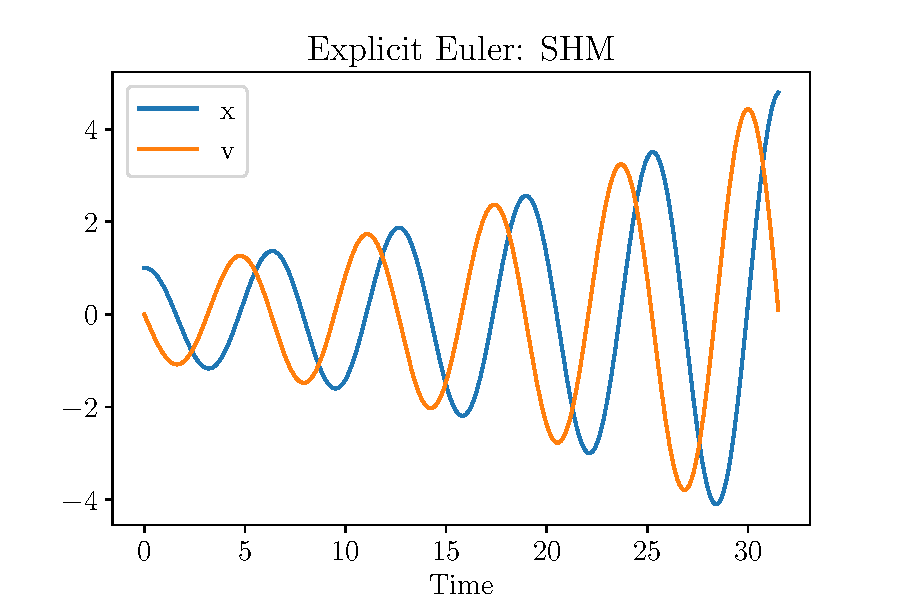
\includegraphics[width=.35\textwidth]{p1_1.pdf}%
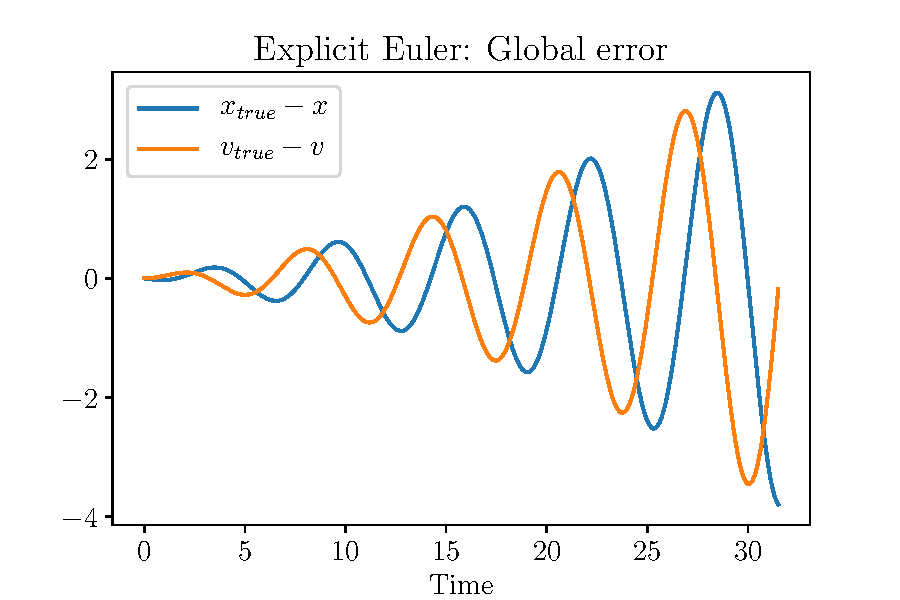
\includegraphics[width=.35\textwidth]{p1_2.pdf}%
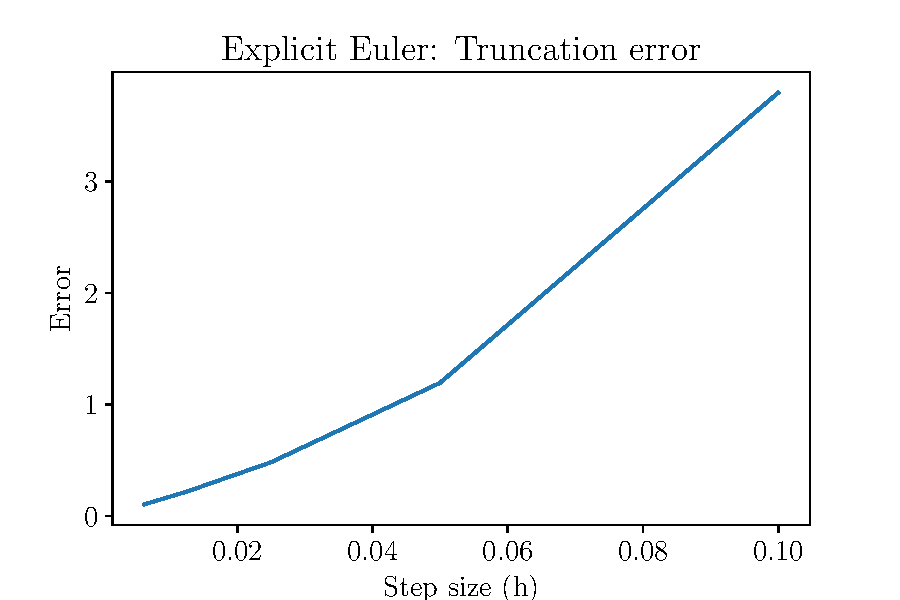
\includegraphics[width=.35\textwidth]{p1_3.pdf}
\\
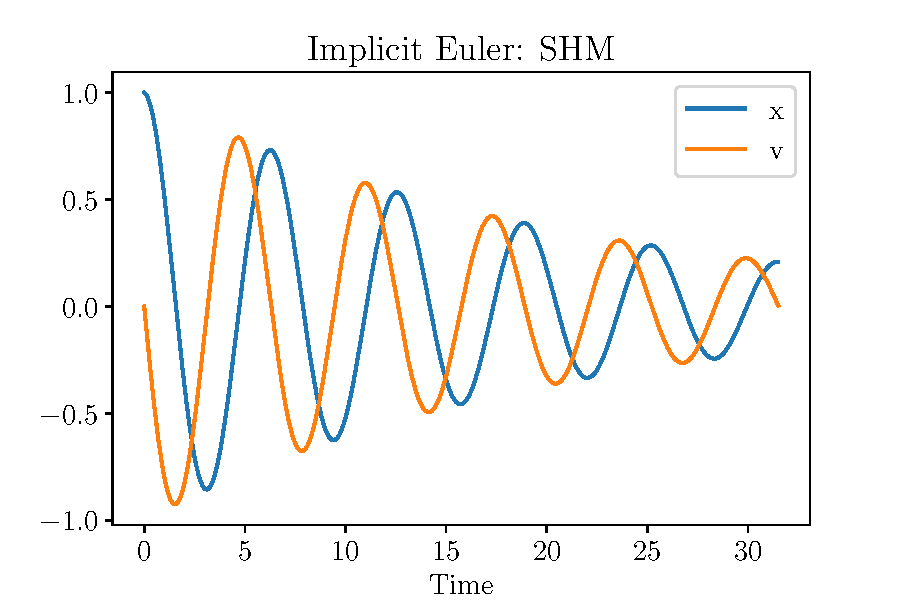
\includegraphics[width=.35\textwidth]{p1_5_1.pdf}%
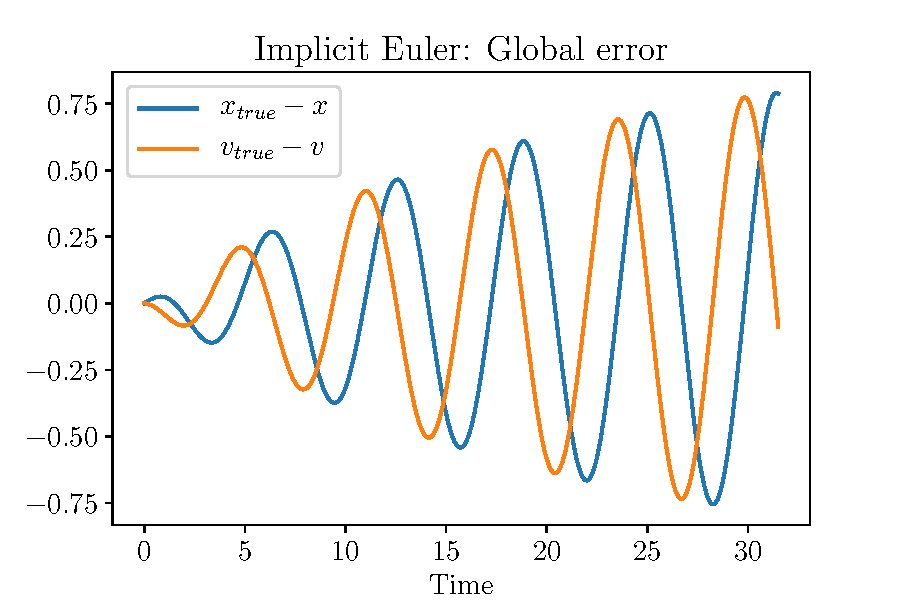
\includegraphics[width=.35\textwidth]{p1_5_2.pdf}%
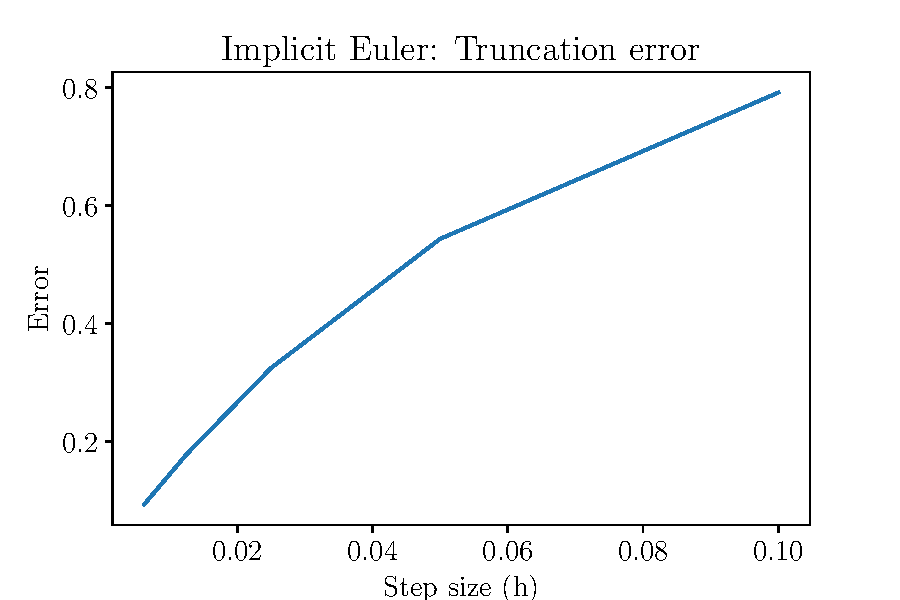
\includegraphics[width=.35\textwidth]{p1_5_3.pdf}
\caption{Euler method approximations of simple harmonic motion with $x_0 = 1$ and $v_0=0$ using a step size of $h=0.1$ unless otherwise specified. The explicit Euler method increasingly overestimates velocity and position over time, while the implicit Euler method underestimates. The global error of the explicit method grows without bound, while the global error of the implicit method approaches the analytic solution as the approximate motion damps to stationary.}
\label{fig:motion}
\end{sidewaysfigure}

\begin{sidewaysfigure}[ht]
\centering
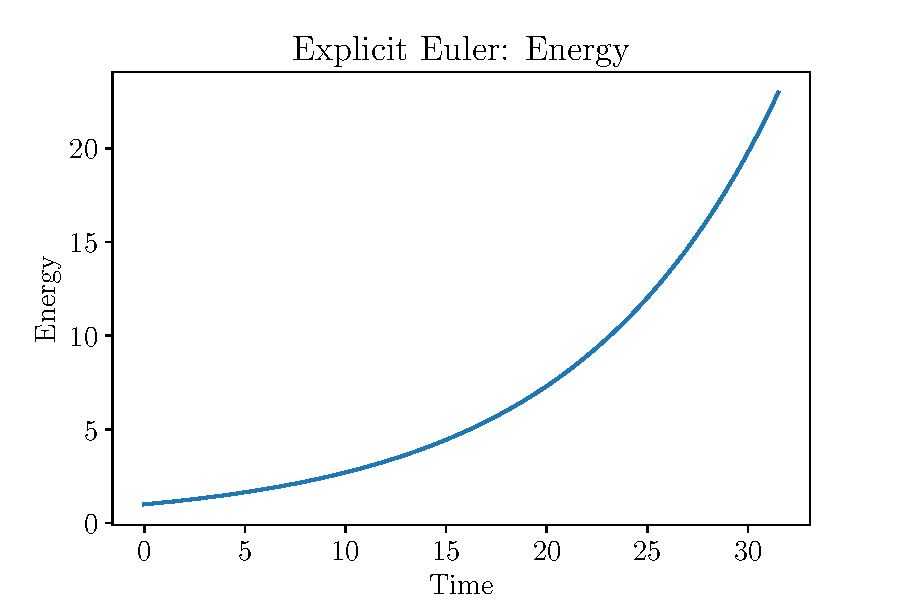
\includegraphics[width=.35\textwidth]{p1_4.pdf}%
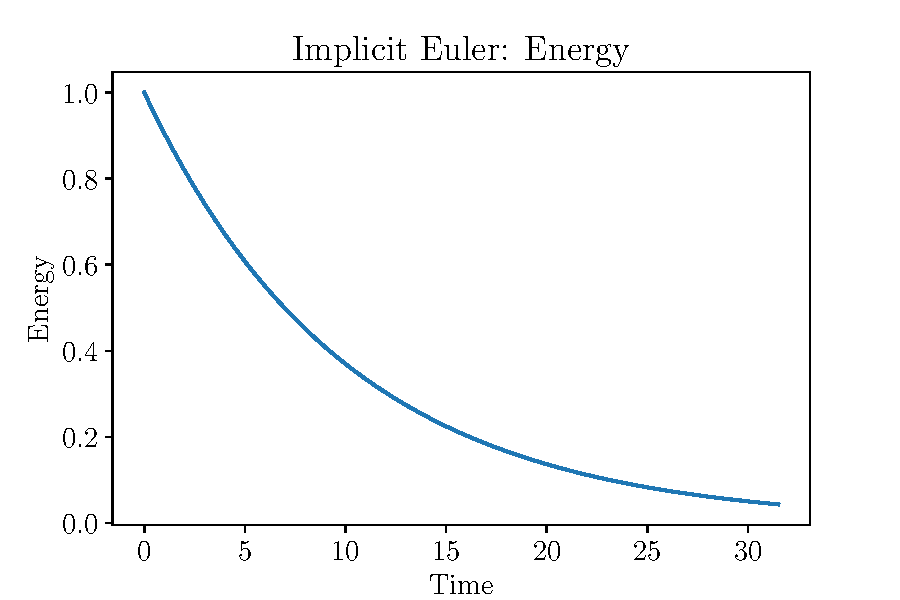
\includegraphics[width=.35\textwidth]{p1_5_4.pdf}%
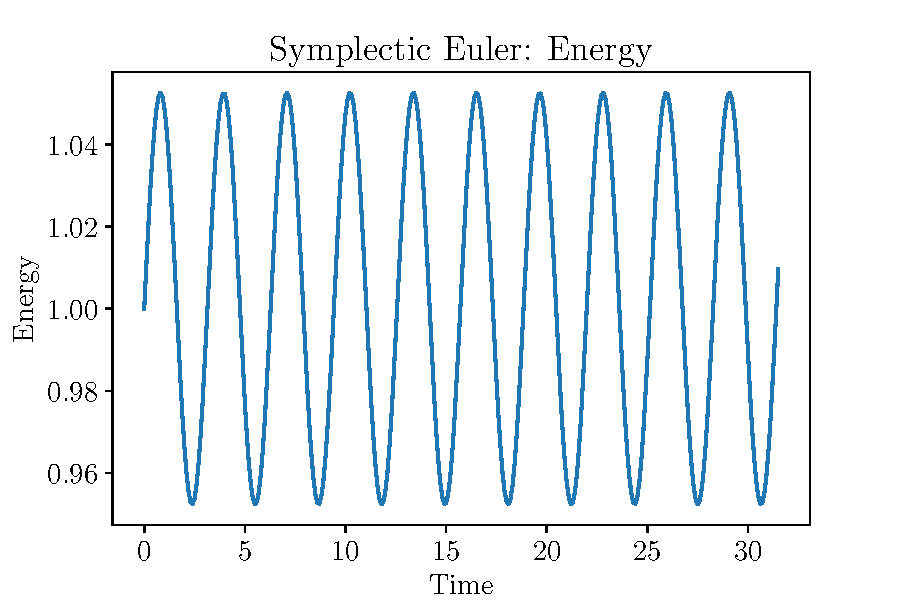
\includegraphics[width=.35\textwidth]{p2_3.pdf}
\\
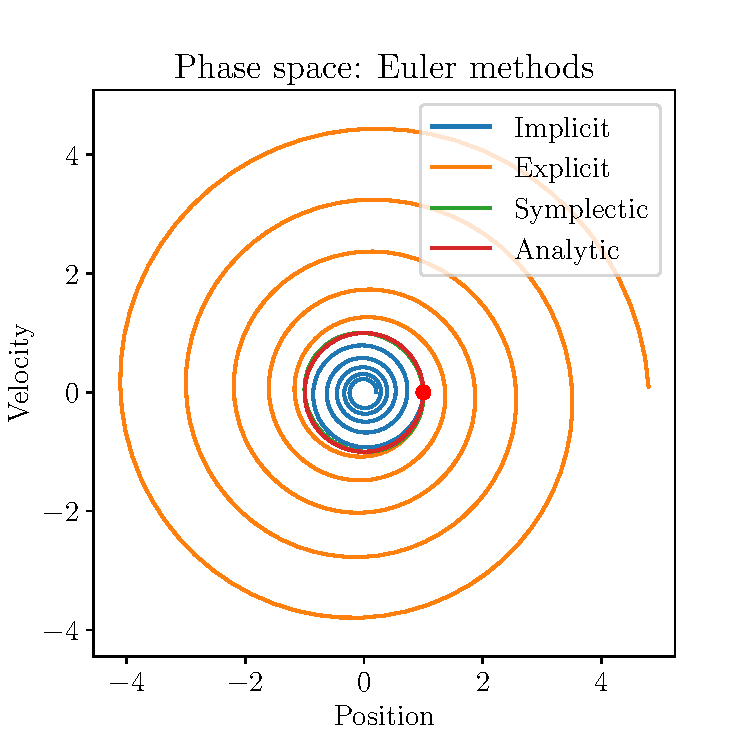
\includegraphics[width=.45\textwidth]{p2_2.pdf}
\caption{Euler method approximations of simple harmonic motion with $x_0 = 1$ and $v_0=0$ using a step size of $h=0.1$. Plotted over 5 periods of oscillation. The explicit method accumulates energy and the implicit method dissipates energy; this is obvious in the phase-space diagram as well. The symplectic method does not conserve energy strictly, but the time-averaged energy is conserved. Unlike the other methods, the symplectic Euler phase-space trajectory is  closed.}
\label{fig:energy}
\end{sidewaysfigure}

\section*{Part 2} 
\subsection*{Exercises 1 \& 2}
The phase-space geometries of the explicit and implicit Euler methods are not closed shapes. The explicit solution spirals \textit{out} while the implicit solution spirals \textit{in}, as expected. However, the symplectic method is indeed a closed loop. Comparing it to the true circular trajectory, it appears that this estimate `wobbles'; that is, the symplectic phase-space trajectory appears to be some closed ellipse. Physically, this conservation of phase-space volume is much more `realistic'.

%%%%%%%%%%%%%%%%%%%%%%%%%%%%%% Exercise 2
\subsection*{Exercise 3}
The total energy estimated by the symplectic Euler method does not grow without bound or dissipate to zero, but instead oscillates around the true constant energy at twice the frequency of the oscillator itself. This is exactly as expected from the phase-space diagram which shows the symplectic trajectory deviating `in' and `out' twice per cycle (i.e. the ellipse crosses the true circular path a total of four times per full motion). 



\section*{Assignment 4}
\subsection*{Makefile}
\verbatiminput{Makefile}

\subsection*{Version control}
\verbatiminput{git.log}


\subsection*{Source}
\verbatiminput{Ph20_Set_3.py}


\end{document}                  
